\section{评估}
\label{socksdirect:sec:evaluation}


%\begin{figure}[htpb]
%	\centering
%	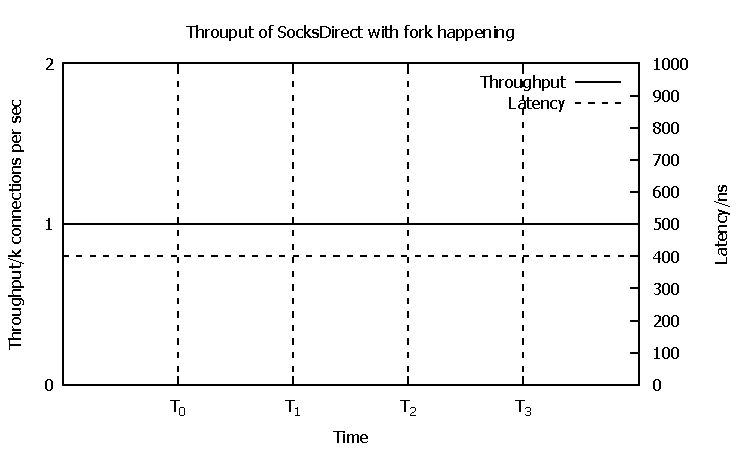
\includegraphics[width=\columnwidth]{eval/microbenchmark/fork-tput.pdf}
%	\caption{Throughput of SocksDirect with fork happening}
%	\label{socksdirect:fig:eval-fork-tput}
%\end{figure}

\sys{} 在三个组件中实现:一个用户空间库 \libipc {} 和一个带有17K行C ++代码的监控守护进程,以及一个支持零拷贝的修改过的RDMA 网卡驱动程序。
本节从以下方面评估\sys{}:

\parab {有效地为主机内套接字使用共享内存。}
对于8字节消息,\sys 实现0.3 $\mu$s RTT和每秒23~M消息的吞吐量。 对于大型消息,\sys 使用零拷贝来实现Linux的1/13延迟和26x吞吐量。

\parab {有效地使用RDMA进行主机间套接字。}
\sys 达到1.7 $\mu$s RTT,接近原始RDMA性能。
零拷贝时,一个连接会使100~Gbps链路饱和。

%\parab{Robust with number of connections.}
%The performance above can be maintained with up to 100 million connections.

%\parab{Corner-case operations does not affect long-term performance.}
%After corner-case operations such as \texttt{fork}, the performance recovers quickly.

\parab {可扩展核心数。}
随着核心数量的增加,吞吐量几乎可以线性扩展。


\parab {使用未经修改的端到端应用程序显着加速。}
例如,\sys  {}将Nginx HTTP请求延迟减少5.5倍到20倍。


\subsection{方法}
\label{socksdirect:subsec:methodology}

本节使用两个Xeon E5-2698 v3 CPU,256~GiB内存和一个Mellanox ConnectX-4网卡评估服务器上的\sys{}。服务器与Arista 7060CX-32S 100G交换机互连 \cite {arista-7060cx}。服务器使用Ubuntu 16.04和Linux 4.15,将RoCEv2用于RDMA协议,每64条消息轮询一次完成队列。
每个线程都固定在CPU内核上。在收集数据之前,进行了足够的预热测试。
对于延迟,本节使用一个乒乓应用程序报告平均往返时间,误差条代表1%和99%百分位数。
对于吞吐量,一方保持发送数据而另一方不断接收数据。
本节将比较Linux,原始RDMA写原语(write verb),Rsocket~ \cite {rsockets}和LibVMA~ \cite {libvma},这是针对Mellanox 网卡优化的用户空间TCP / IP堆栈。
本节没有评估mTCP~ \cite {jeong2014mtcp},因为底层DPDK库对Mellanox ConnectX-4网卡的支持有限。由于批处理,mTCP具有比RDMA高得多的延迟,报告的吞吐量为每秒1.7~M包~~ \cite {kalia2018datacenter}。

\subsection{微基准测试}
\label{socksdirect:subsec:microbenchmark}

\subsubsection{延迟和吞吐量}



图 \ref {socksdirect:fig:eval-msgsize-intra}显示了一对发送方和接收方线程之间的主机内套接字性能。
对于8字节消息,\sys 实现0.3 $ \mu $ s往返延迟(Linux的1/35)和每秒23~M消息吞吐量(Linux的20倍)。
相比之下,一个简单的SHM队列具有0.25 $ \mu $ s往返延迟和27~M吞吐量,表明\sys 增加了很少的开销。
RSocket具有6x延迟和1/4吞吐量的\sys  {},因为它使用网卡转发主机内数据包,这会导致PCIe延迟。
LibVMA只是将内核TCP套接字用于主机内部。
\sys  {}的单向延迟为0.15 $ \mu $ s,甚至低于内核交叉(0.2 $ \mu $ s)。基于内核的套接字需要在发送方和接收方都进行内核交叉。


由于内存复制,对于8~KiB消息,\sys 的吞吐量仅比Linux高60%,延迟低4倍。对于大小至少为16~KiB的消息,\sys 使用页面重映射来实现零拷贝。
对于1~miB消息,\sys 比Linux具有1/13延迟和26x吞吐量。
由于事件通知延迟,RSocket的延迟不稳定,在某些情况下甚至可能比Linux大。



\begin{figure*}[htbp]
	\centering
	\subfloat[单机内吞吐量。]{                    
		%\begin{minipage}{0.4\textwidth}
		\centering
		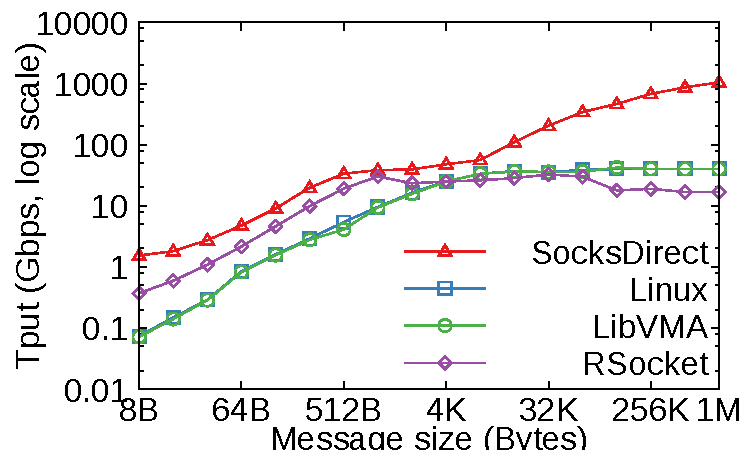
\includegraphics[width=0.5\textwidth]{eval/microbenchmark/msgsize-ipc-tput.pdf}
		\label{socksdirect:fig:eval-msgsize-ipc-tput}
		%\end{minipage}
	}
	\subfloat[单机内延迟。]{
		%\begin{minipage}{0.4\textwidth}
		\centering 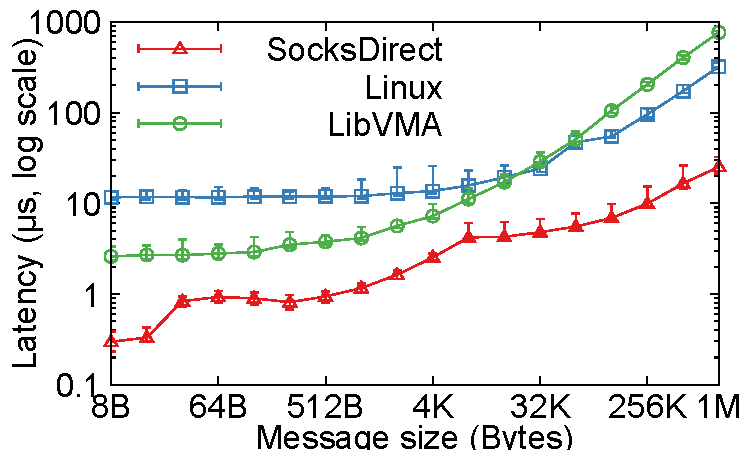
\includegraphics[width=0.5\textwidth]{eval/microbenchmark/msgsize-ipc-lat.pdf}
		\label{socksdirect:fig:eval-msgsize-ipc-lat}
		%\end{minipage}
	}
	
	\caption{不同消息大小下的单机内通信单核消息性能。}
	\label{socksdirect:fig:eval-msgsize-intra}
\end{figure*}


图 \ref {socksdirect:fig:eval-msgsize-inter}显示了一对线程之间的主机间套接字性能。
对于8字节消息,\sys 实现每秒18M消息吞吐量(Linux的15倍)和1.7微秒/秒的延迟(Linux的1/17)。
吞吐量和延迟接近原始RDMA写操作(如虚线所示),它没有套接字语义。
由于批处理,\sys  {}对于8字节消息的吞吐量甚至高于RDMA。
对于16到128字节的消息,LibVMA还使用批处理来实现比\sys  {}更好的吞吐量,但延迟是\sys  {}的7倍。
对于小于8~KiB的消息大小,主机间RDMA的吞吐量略低于主机内SHM,因为环形缓冲区结构是共享的。
对于512B到8KiB消息,\sys  {}受数据包复制的限制,但由于缓冲管理开销减少,仍然比RSocket和LibVMA更快。
对于零拷贝消息($\ge$ 16 KiB),\sys  {}使网络带宽饱和,其具有所有比较工作的3.5倍吞吐量和RSocket的72%延迟。


\begin{figure*}[htbp]
	\centering
	\subfloat[跨主机吞吐量。]{
		%\begin{minipage}{0.4\textwidth}
		\centering 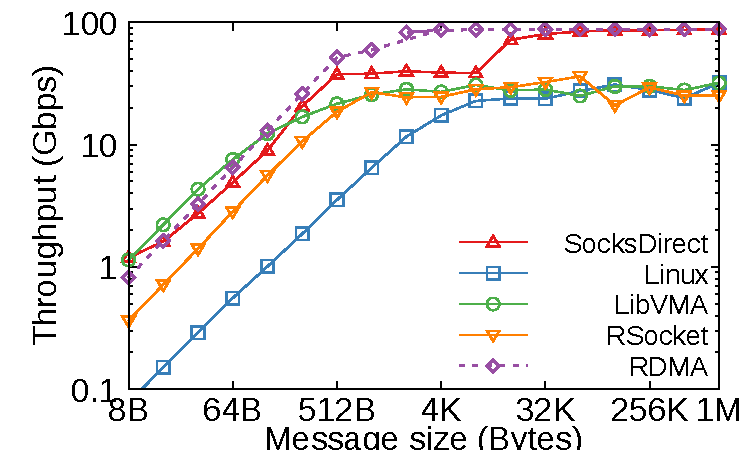
\includegraphics[width=0.5\textwidth]{eval/microbenchmark/msgsize-network-tput.pdf}
		\label{socksdirect:fig:eval-msgsize-network-tput}
		%\end{minipage}
	}
	\subfloat[跨主机延迟。]{
		%\begin{minipage}{0.4\textwidth}
		\centering 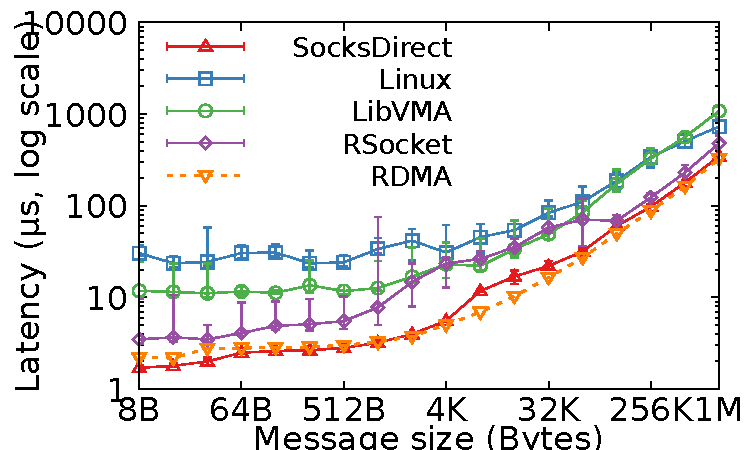
\includegraphics[width=0.5\textwidth]{eval/microbenchmark/msgsize-network-lat.pdf}
		\label{socksdirect:fig:eval-msgsize-network-lat}
		%\end{minipage}
	}
	
	\caption{不同消息大小下的跨主机通信单核消息性能。}
	\label{socksdirect:fig:eval-msgsize-inter}
\end{figure*}




\subsubsection{多核可扩放性}

%Figure~\ref{socksdirect:fig:eval-connnum-tput} shows the throughput with different number of concurrent connections.
%We establish connections between two processes before testing, then send and receive data from the connections in a round-robin order.
%\sys  can support more than 100 million concurrent connections with 16~GiB of memory, and the throughput does not degrade under such high concurrency.
%\sys  achieves connection stability by multiplexing connections via a single queue.
%In comparison, the performance of RDMA, LibVMA and Linux drops quickly as the number of connections increase. There is a sharp performance drop with more than 512 RDMA connections, because the RDMA transport states saturate the 网卡 cache. Although LibVMA and Linux do not use RDMA as transport, they maintain per-文件描述符 buffers, which lead to CPU cache and TLB miss with thousands of connections. Furthermore, LibVMA installs flow steering rules to 网卡 for each connection, which also leads to 网卡 cache miss.




\sys 实现了主机内和主机间套接字的几乎线性可扩展性。
对于主机内套接字,\sys 在16对发送器和接收器核心之间提供每秒306~M消息的吞吐量,这是Linux的40倍和RSocket的30倍。
LibVMA回退到Linux用于主机内套接字。
使用RDMA作为主机间套接字,\sys 使用批处理以16个内核实现每秒276~M个消息的吞吐量,这是本章使用的RDMA网卡的消息吞吐量的2.5倍。
由于缓冲区管理的可扩展性有限,RSocket的主机内部为24~M,主机间为33~M。
由于共享网卡队列上的锁争用,与单线程相比,LibVMA的吞吐量减少到两个线程的1/4,而三个和更多线程的1/10。
Linux吞吐量从1到7个核心线性扩展,并在环回或具有更多核心的网卡队列上出现瓶颈。


\begin{figure*}[htbp]
	\subfloat[单机内吞吐量。]{                    
		%\begin{minipage}{0.4\textwidth}
		\centering
		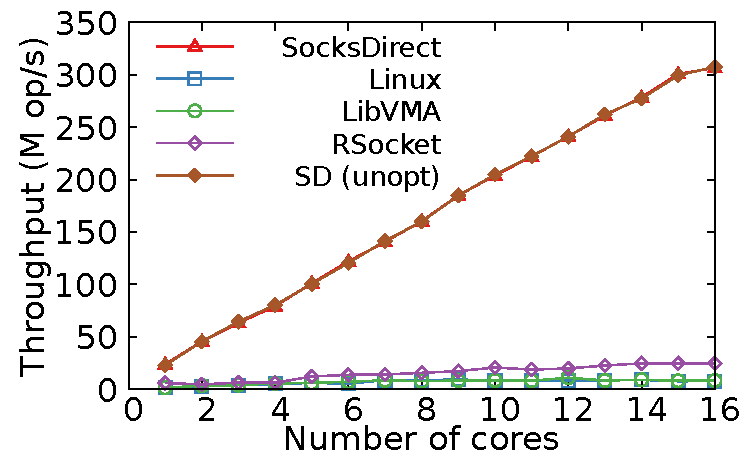
\includegraphics[width=0.5\textwidth]{eval/microbenchmark/corenum-IPC-tput.pdf}
		\label{socksdirect:fig:eval-cornum-ipc}
		%\end{minipage}
	}
	\subfloat[跨主机吞吐量。]{
		%\begin{minipage}{0.4\textwidth}
		\centering 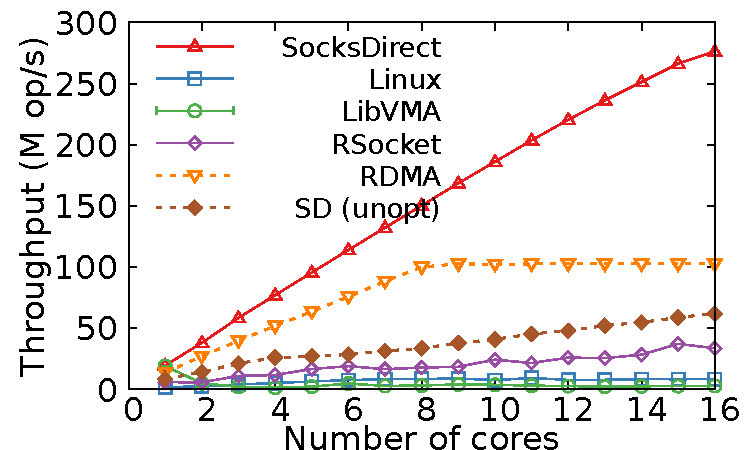
\includegraphics[width=0.5\textwidth]{eval/microbenchmark/corenum-network-tput.pdf}
		\label{socksdirect:fig:eval-cornum-network}
		%\end{minipage}
	}
	
	\caption{不同 CPU 核数下的 8 字节消息吞吐量。}
	\label{socksdirect:fig:eval-corenum-tput}
\end{figure*}


%The multi-thread scalability of \sys  attributes to the partitioning of states and removal of synchronization.
%We can also see that shared memory communication has 5x throughput than RDMA.% Using RDMA 网卡 for intra-host socket would meet this bottleneck and thus not scalable.

%Figure~\ref{socksdirect:fig:eval-conn-setup-tput} shows the throughput of connection creation with different number of cores. Each core can create 1.4~M new connections per second, which is 20x of Linux and 2x of mTCP~\cite{jeong2014mtcp}. The upper bound is 5.3~M connections per second, where the monitor becomes a bottleneck.

最后评估共享核心的多个线程的性能。 每个线程都需要等待轮到它来处理消息。
如图 \ref {socksdirect:fig:eval-context-switch}所示,尽管消息处理延迟几乎与活动进程的数量呈线性增长,但它仍然是Linux的1/20到1/30。


\begin{figure}[htbp]
	%\centering
	%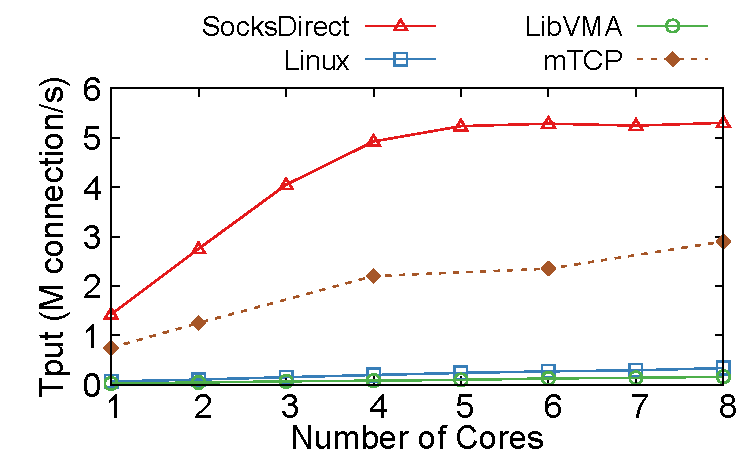
\includegraphics[width=\textwidth]{eval/microbenchmark/conn-setup-tput.pdf}
	%
	%\caption{Connection creation throughput with number of cores.}
	%\label{socksdirect:fig:eval-conn-setup-tput}
	
	%\begin{minipage}{0.4\textwidth}
	\centering 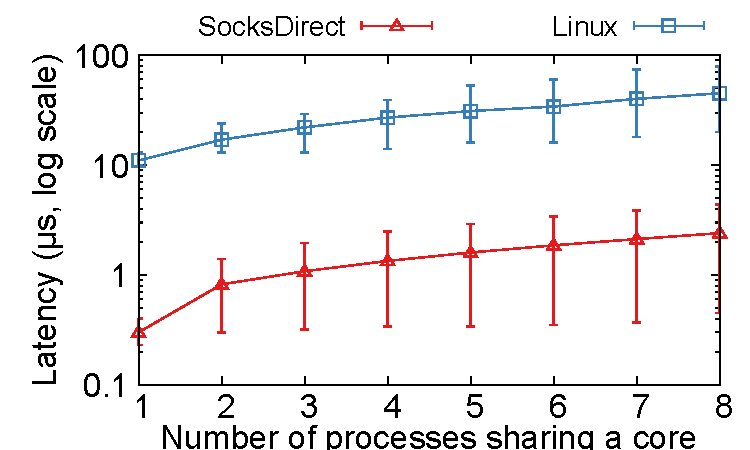
\includegraphics[width=0.5\textwidth]{eval/microbenchmark/sharecore-lat.pdf}
	
	\caption{多进程共享 CPU 核的消息处理延迟。}
	\label{socksdirect:fig:eval-context-switch}
	%\end{minipage}
\end{figure}

\iffalse
\begin{figure*}[htbp]
	\centering
	\subfloat[单机内吞吐量。]{                    
		%\begin{minipage}{0.4\textwidth}
		\centering
		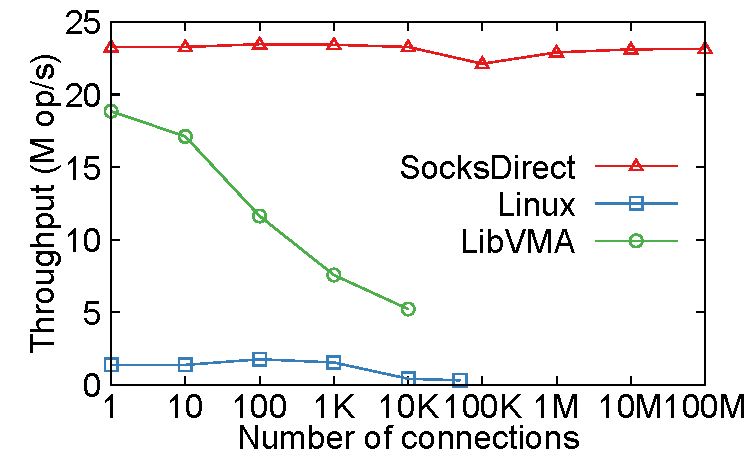
\includegraphics[width=0.5\textwidth]{eval/microbenchmark/connnum-ipc-tput.pdf}
		\label{socksdirect:fig:eval-connnum-ipc-tput}
		%\end{minipage}
	}
	\subfloat[跨主机吞吐量。]{
		%\begin{minipage}{0.4\textwidth}
		\centering 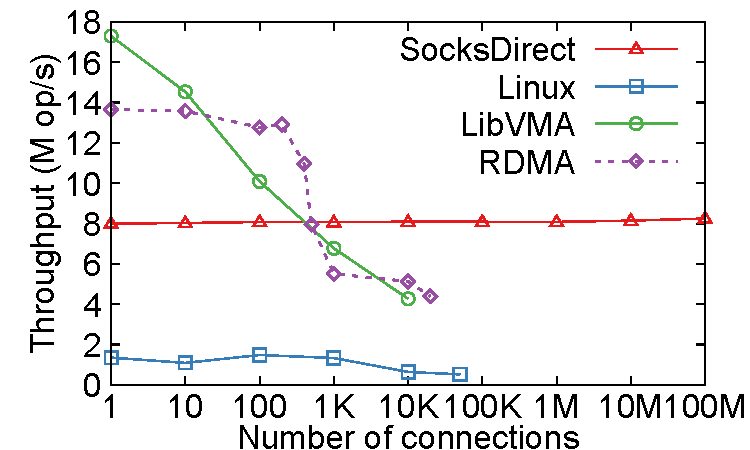
\includegraphics[width=0.5\textwidth]{eval/microbenchmark/connnum-network-tput.pdf}
		\label{socksdirect:fig:eval-connnum-network-tput}
		%\end{minipage}
	}
	
	\caption{不同并发连接数量下的单核吞吐量。}
	\label{socksdirect:fig:eval-connnum-tput}
\end{figure*}
\fi

%Finally, we benchmark the throughput and latency after \texttt{fork} and other corner-case operations. Initially, there is only one pair of sender and receiver. At time $T_0$, receiver forks, and the parent process keeps receiving. At time $T_1$, the child process begins to receives takes over the socket. At time $T_2$, sender forks, and only the parent sends. At time $T_3$, the child sender also starts sending. We find that both throughput and latency resume to initial maximal performance within 1~ms after each event.
